\section{Confounds, honest disclosure, and analysis}
\label{sec:confounds}

The experiments support a selective deployment method, not a broad UV optimizer. This section makes the confounds explicit: what the accepted gains do not depend on, what they do depend on, and where the current evidence is weak.

\subsection{Strict matched controls}
\label{sec:matched_controls}

\begin{table}[t]
\centering
\scriptsize
\caption{Strict matched-control results. (a) The gain survives atlas-size, padding, and chart-count locks, but disappears under distortion, utilization, or all-lock protocols. (b) Absolute UV-proxy changes for the accepted cases: Q$_{95}$ distortion stays within $\pm$25\% but texture utilization drops 35--60\%; chart count and seam length are unchanged. This quantifies the localized UV-proxy cost the C5 gate is willing to pay for the +10--15 dB PBR gain.}
\label{tab:matched}
\begin{tabular}{@{}lrrll@{}}
\toprule
\multicolumn{5}{@{}l}{\textbf{(a) Relit PSNR delta under matched controls}}\\
Condition & Spot $\Delta$ & Bunny $\Delta$ & matched OK & C5 \\
\midrule
Atlas-size and padding locked & \textbf{+14.67} & \textbf{+10.23} & yes & accept \\
Chart count locked within +/-5\% & \textbf{+14.67} & \textbf{+10.23} & yes & accept \\
Distortion Q95 locked & +0.00 & +0.00 & yes & rollback \\
Texture utilization locked & +0.00 & +0.00 & yes & rollback \\
All strict matched controls & +0.00 & +0.00 & yes & rollback \\
\bottomrule
\end{tabular}

\vspace{0.4em}
\begin{tabular}{@{}lrrrr@{}}
\toprule
\multicolumn{5}{@{}l}{\textbf{(b) Absolute UV-proxy stats for accepted cases (init $\rightarrow$ deployed)}}\\
Asset & $Q_{95}$ distortion & Utilization & Charts & Seam length \\
\midrule
spot/PartUV & 63.80 $\rightarrow$ 62.90 & 0.382 $\rightarrow$ 0.236 & 19 $\rightarrow$ 19 & 22.20 $\rightarrow$ 22.20 \\
bunny/PartUV & 11.02 $\rightarrow$ 13.56 & 0.634 $\rightarrow$ 0.263 & 2 $\rightarrow$ 2 & 11.06 $\rightarrow$ 11.06 \\
\bottomrule
\end{tabular}
\end{table}


\begin{figure}[t]
  \centering
  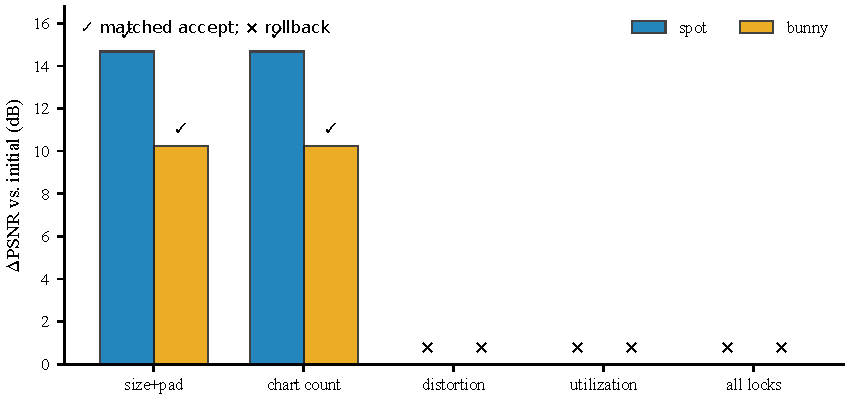
\includegraphics[width=0.95\linewidth]{figures/main/fig5_matched.pdf}
  \caption{Strict matched controls for the accepted PartUV cases. Gains persist when atlas size, padding, or chart count are locked, but vanish under distortion, utilization, or all strict matched controls, indicating a principled downstream-fidelity trade-off.}
  \label{fig:matched_control}
\end{figure}

\Cref{tab:matched,fig:matched_control} rule out three simple explanations. The spot and bunny gains persist when atlas size and padding are locked, and they also persist when chart count is locked within the matched protocol. The method is therefore not merely buying a larger texture, adding padding, or increasing chart count.

The same table also shows the cost of the method. When distortion \(Q_{95}\), packing utilization, or all strict controls are locked, both accepted PartUV cases roll back to baseline. The gain requires localized freedom in distortion and utilization. We interpret this as a principled trade-off: classical UV metrics are useful proxies for atlas geometry and packing efficiency, but they are not equivalent to downstream PBR relighting fidelity. The method spends distortion/utilization slack only when the residual evidence and C5 gate justify the exchange.

\paragraph*{Semantic preservation.}
\begin{table}[t]
\centering
\caption{Chart-part purity comparison (\cref{sec:confounds}). PartUV and our repaired output preserve part semantics perfectly relative to the PartUV part hierarchy; xatlas re-charting reduces purity, with entropy growing on assets that have many small parts.}
\label{tab:purity}
\begin{tabular}{@{}lrrrr@{}}
\toprule
Asset & xatlas Purity & PartUV Purity & Ours Purity & xatlas Entropy \\
\midrule
spot & 0.878 & \textbf{1.000} & \textbf{1.000} & 0.079 \\
bunny & 0.866 & \textbf{1.000} & \textbf{1.000} & 0.509 \\
objaverse & 0.783 & \textbf{1.000} & \textbf{1.000} & 0.594 \\
\bottomrule
\end{tabular}
\end{table}

Chart--part purity gives a quantitative reason not to replace PartUV with xatlas when part organization is a pipeline constraint. Using the PartUV leaf-chart partition as the reference part proxy, xatlas purity is lower on spot, bunny, and the Objaverse asset, while PartUV and our repaired output remain at the reference purity. \emph{This metric is partition-dependent}: by construction, our repair never globally re-charts, and PartUV is taken as the reference partition, so the purity comparison is a direct check of whether xatlas's global re-charting violates the chosen partition. It is therefore a witness for "does PartUV-style chart organization survive repair?" rather than a venue-independent editability score; we treat human-labeled part purity, downstream rig-aware editing, and accessory transfer benchmarks as future evaluation work.

To avoid relying only on the PartUV-derived reference partition, we add the curvature-alignment metric in \cref{tab:curvature_alignment}. It treats high-dihedral mesh edges as a geometry-only proxy for part-like boundaries and computes chart-boundary IoU/precision against that set. This metric still is not a human editing benchmark, but it removes the tautology that PartUV-defined parts automatically favor PartUV-preserving repairs.

\subsection{Selective trigger rate}
\label{sec:selective_trigger}

Across the 12 Main Anchor Evaluation cases and eight Transfer and Robustness Study transfer cases, C5 accepts three repairs and rolls back 17 candidates. The accepted cases are spot/PartUV, bunny/PartUV, and procedural warped cylinder, giving a 3/20 trigger rate over the displayed tested rows. The A1 key-case rerun in \cref{tab:a1_split} separately checks two accepted PartUV cases (spot, bunny) and two rollback controls (spot/xatlas, Objaverse/xatlas) across three disjoint proposal/gate/test split seeds. Accepted PartUV gains persist on the held-out test split (spot $+12.58 \pm 0.83$ dB, bunny $+11.84 \pm 0.89$ dB), and the rollback controls stay at $\Delta = 0.00 \pm 0.00$ dB across all three seeds, so the headline gain is not an artifact of evaluating on the same residual signal that drove repair selection. This is a leakage-control audit rather than a replacement for the full single-seed table. The discrepancy between candidates and deployed outputs is deliberate: the method is allowed to search, but deployment is gated. This matters most for already-good xatlas rows and for procedural transfer rows where a high-PSNR candidate can still violate seam, distortion, or utilization guards. Those candidates are not deployed.

\begin{figure}[t]
  \centering
  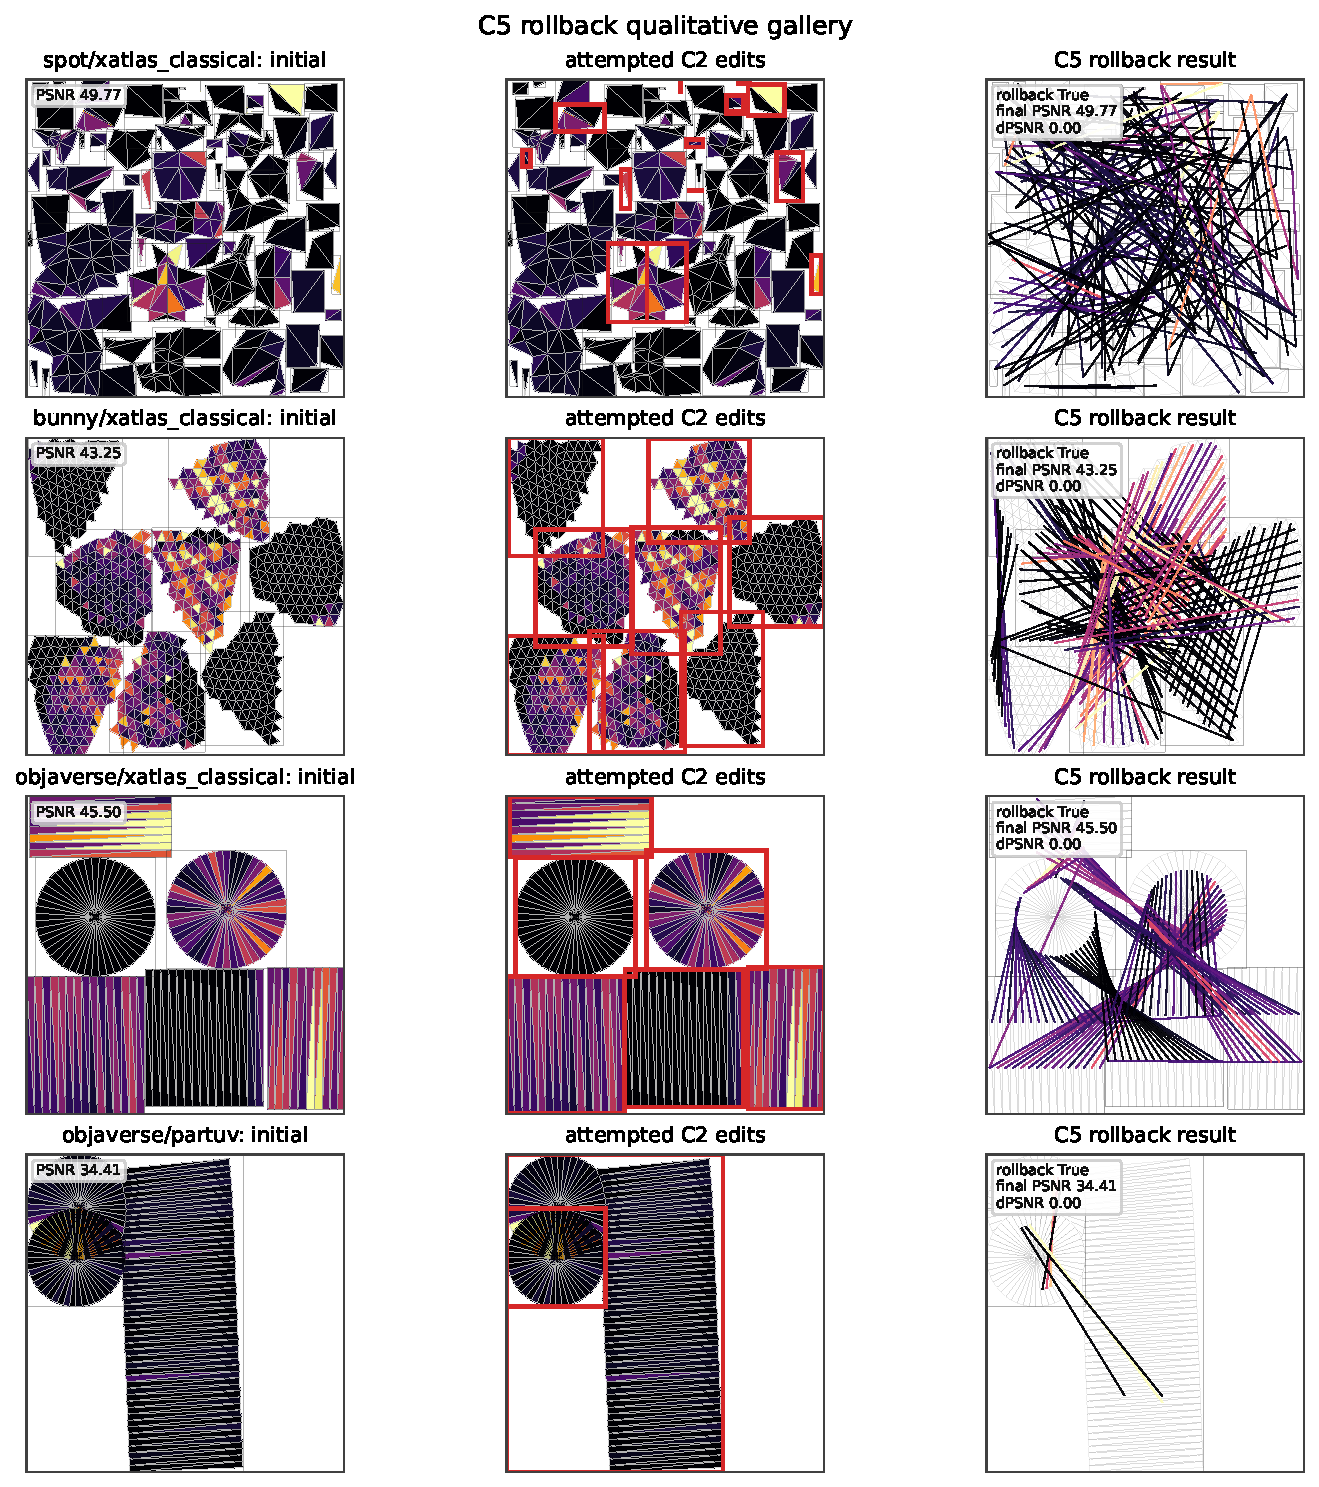
\includegraphics[width=0.95\linewidth]{figures/qualitative_residual_chain/rollback_gallery.pdf}
  \caption{Rollback gallery. The method can propose edits for cases where the residual atlas suggests a possible repair, but C5 deploys the baseline when held-out relighting and seam metrics do not justify the change.}
  \label{fig:rollback_gallery}
\end{figure}

\Cref{fig:rollback_gallery} visualizes this non-harm behavior. It is not evidence that every attempted edit is visually useful; it is evidence that failed candidates can be filtered out before deployment.

\subsection{C4 and weak isolated signals}
\label{sec:c4_disclosure}

C4 is included because PBR seams are cross-channel: albedo, normal, roughness, and metallic discontinuities are not perceptually interchangeable. However, the present ablations do not prove C4 as a standalone necessary component. A5 and A9 are zero-signal in the completed table, and the current hooks may not isolate channel coupling cleanly. We therefore keep C4 as a diagnostic regularizer and reporting tool rather than a top-level claim. The stronger channel evidence comes from A2, where collapsing the baker to RGB-only loses about 12.5 dB.

\subsection{Baseline reproduction scope}
\label{sec:baseline_scope}

The baseline story is intentionally bounded. The main table uses xatlas, Blender Smart UV, real PartUV, and a matched oracle. FlexPara was blocked by Python/PyTorch/CUDA-op/checkpoint constraints, OT-UVGS was treated as an unverified adjacent capacity idea rather than a direct mesh-UV reproduction, and Flatten Anything and ParaPoint were not fully runnable in the available environment. These failures are not hidden; \cref{app:baseline_failure} gives the reproduction table used to scope the claims.

\subsection{Noise anomaly}
\label{sec:noise_anomaly}

The robustness sweep contains a non-monotonic mesh-noise anomaly. At \(\sigma=0.01\), the spot/PartUV case rolls back and PSNR stays at the baseline 33.35 dB; at \(\sigma=0.02\) and \(\sigma=0.05\), the method accepts and recovers high PSNR (46.28 and 46.71 dB). The PartUV chart count grows monotonically with noise (19, 22, 23, 25 charts for \(\sigma\in\{0,0.01,0.02,0.05\}\)) and the baseline \(Q_{95}\) distortion is in the same range (59--64) across all four cells, so the anomaly is not driven by a structural break in the upstream atlas family. The mechanism is more local: at \(\sigma=0.01\), the C2 candidate's chart count and \(Q_{95}\) distortion are bit-identical to the baseline (22 charts, \(Q_{95}=59.03\)), meaning the residual signal was not concentrated enough to motivate any chart-level action and the candidate is just the baseline atlas reproduced; C5 then correctly rolls back. At \(\sigma=0.02\) and \(\sigma=0.05\) the residual structure exceeds the C2 selection threshold (\cref{eq:topk}), the candidate moves \(Q_{95}\) by +2.0 and +0.8 respectively under the same chart count, and C5 accepts. The anomaly is therefore consistent with a small-noise dead zone in the C2 selection rule rather than a C5 gate fluke or a method failure under deployment; \cref{tab:robustness} retains the row so this dead zone is visible to the reader. Closing this gap would require lowering the C2 top-K threshold for noise-perturbed meshes, which is intentionally not done in this submission because the protocol fixes all C2/C3/C5 thresholds a priori (\cref{sec:implementation}).
